% \begin{figure}[t]
%     \centering
%     \begin{subfigure}[b]{0.32\textwidth}
%         \centering
%         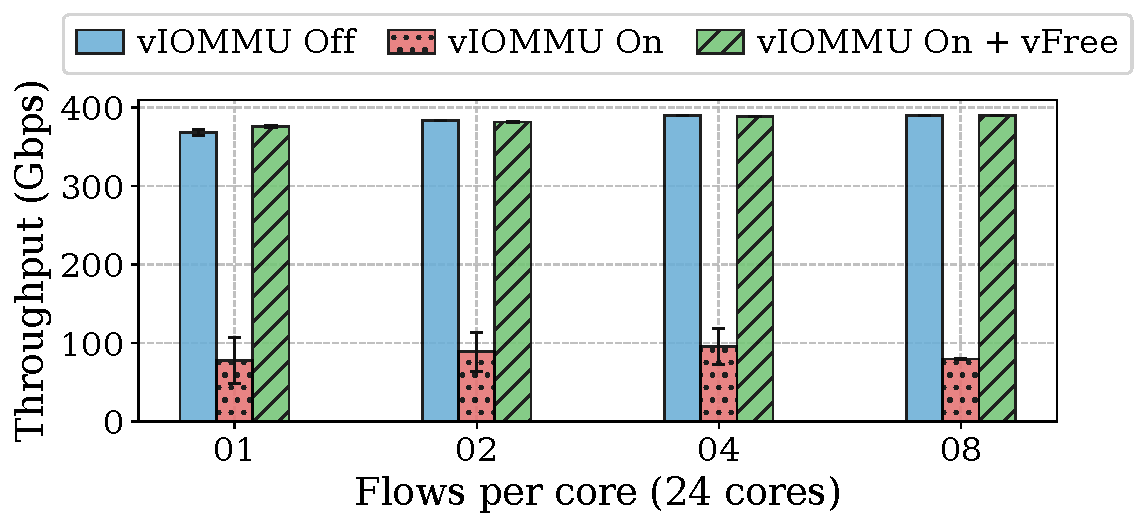
\includegraphics[width=\textwidth]{figures/stress_exp-tput.pdf}
%         \caption{Throughput}
%         \label{vfree:fig:stress-tput}
%     \end{subfigure}
%     \hfill
%     \begin{subfigure}[b]{0.32\textwidth}
%         \centering
%         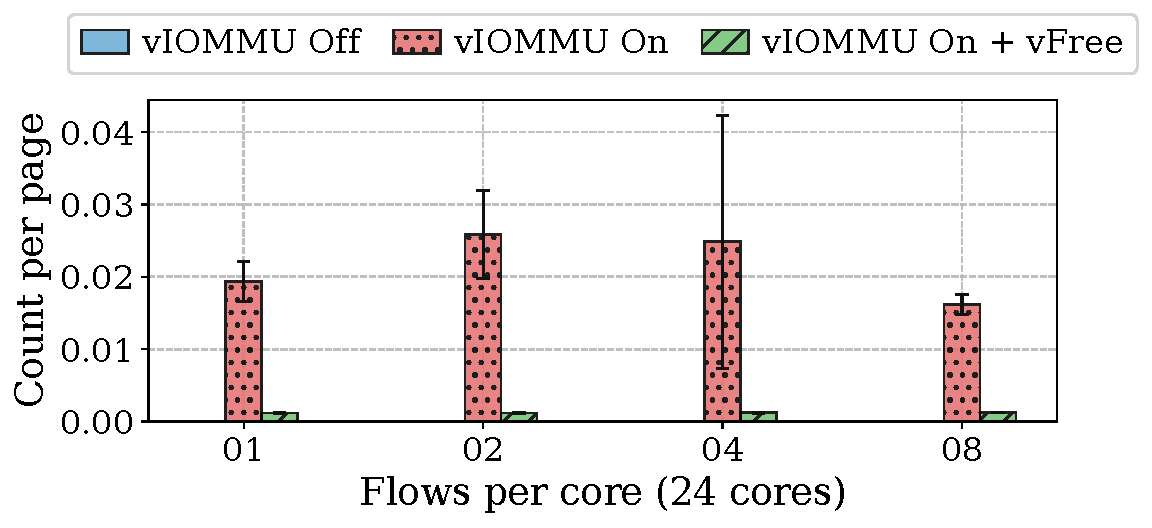
\includegraphics[width=\textwidth]{figures/stress_exp-qi_submit_sync-count_per_page.pdf}
%         \caption{IR-SUB count per page}
%         \label{vfree:fig:stress-qi}
%     \end{subfigure}
%     % \begin{subfigure}[b]{0.32\textwidth}
%     %     \centering
%     %     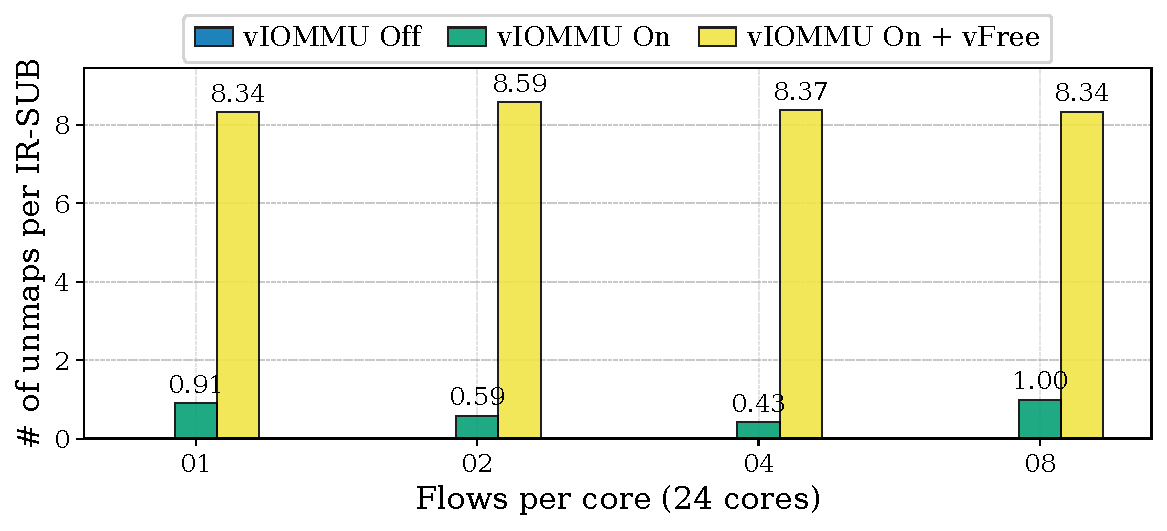
\includegraphics[width=\textwidth]{figures/stress_exp-unmap_to_qi_submit_ratio.pdf}
%     %     \caption{Number of unmap calls per IR-SUB}
%     %     \label{vfree:fig:stress-qi}
%     % \end{subfigure}
%     \hfill
%     \begin{subfigure}[b]{0.32\textwidth}
%         \centering
%         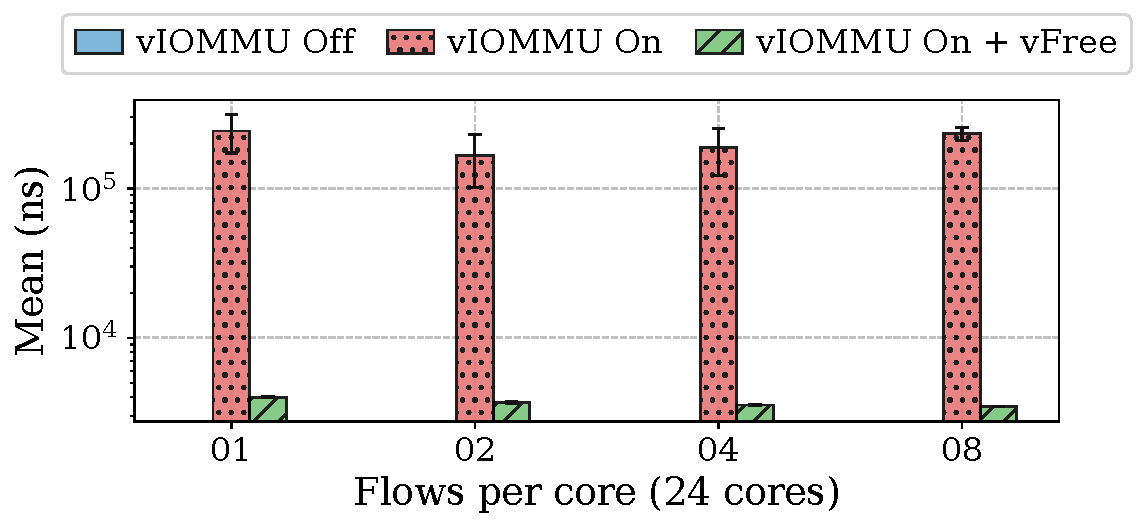
\includegraphics[width=\textwidth]{figures/stress_exp-cache_tag_flush_range-mean_ns.pdf}
%         \caption{IOTLB invalidation overhead per unmap}
%         \label{vfree:fig:stress-flush}
%     \end{subfigure} 
%     \caption{Rx stress test (multiple flows per core): \vfreename{} consistently matches vIOMMU-off throughput.
%     }
%     \label{vfree:fig:stress}
% \end{figure}

% \begin{figure}[t]
%     \centering
%     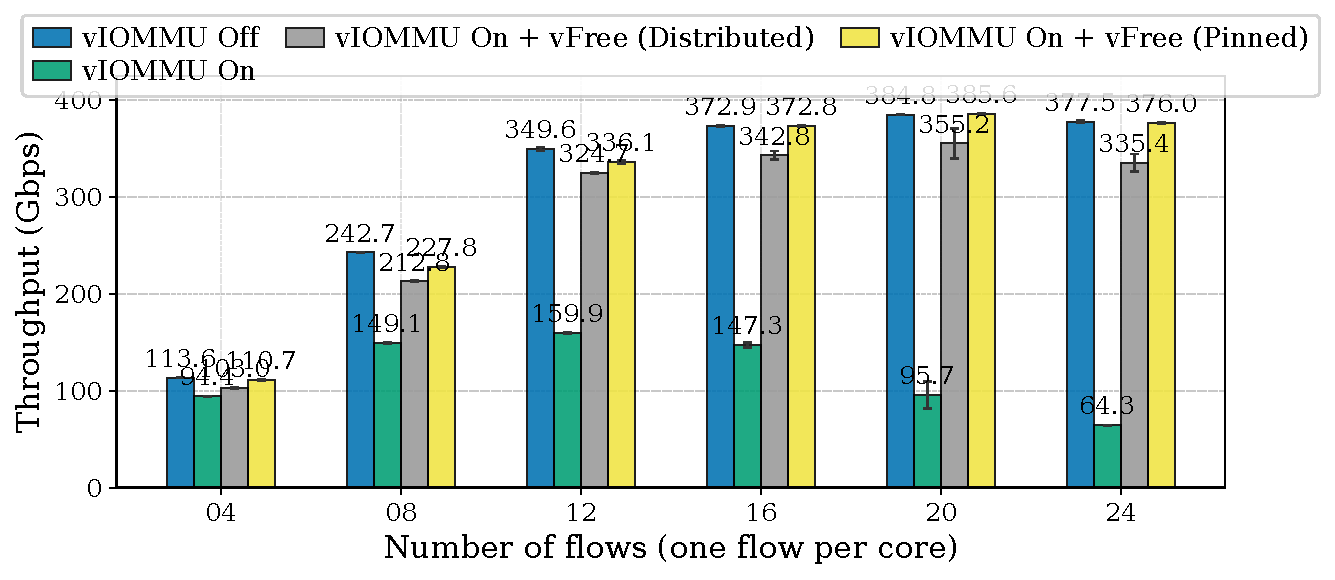
\includegraphics[width=\columnwidth]{figures/eval_core_exp_dlf-tput.pdf}
%     \caption{Rx throughput with DLF.\todo{Rerun with DLF (we should hit 400Gbps)}}
%     \label{vfree:fig:eval-core-dlf}
% \end{figure}

% \begin{figure}[t]
%     \centering
%     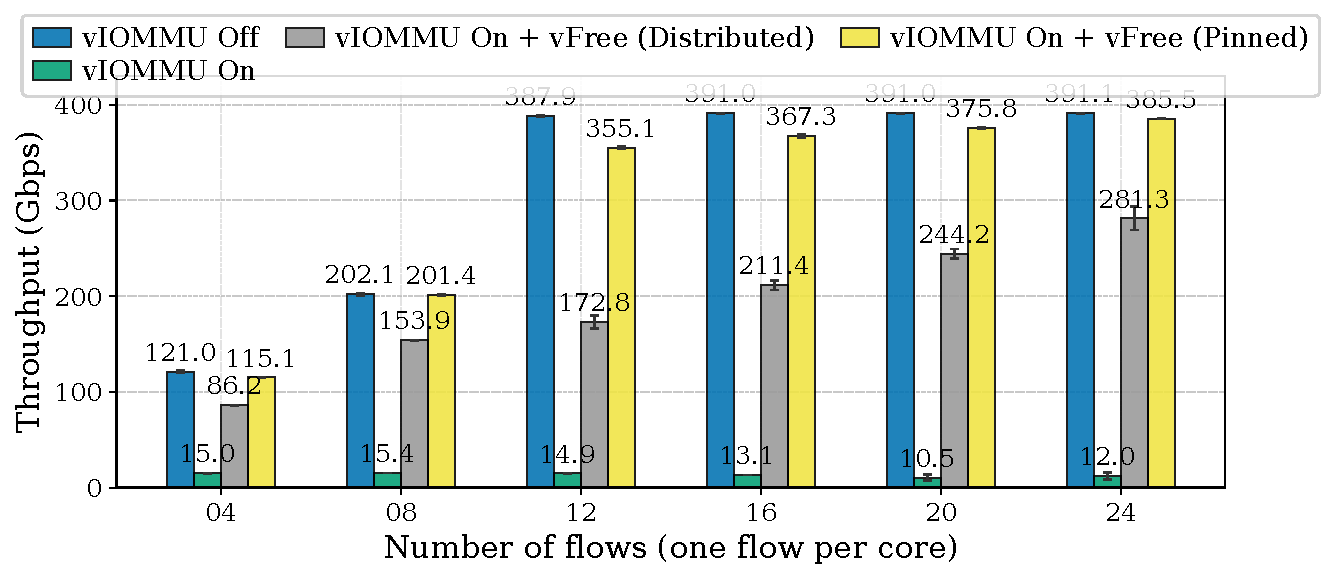
\includegraphics[width=\columnwidth]{figures/tx-ebpf-dlf-tput.pdf}
%     \caption{Tx throughput with DLF.\todo{This is the best we have now}}
%     \label{vfree:fig:tx-dlf}
% \end{figure}

\subsection{Appendix}
\subsubsection{Threat Model}
\label{vfree:sec:threat_model}

Modern OSes typically offer two modes of IO memory protection. 
The strongest guarantee is that of so-called strict mode~\cite{nadav2010iommu, Amit2011vIOMMU} 
% \vfreebrand maintains strict IO memory protection provided by 
    % Linux's strict mode~\cite{} 
    which enforces  
    the free-after-invalidation invariant to ensure % I assume it's the invariant was made early in the design
    \emph{no page can be freed with a stale entry 
        that permits access to the page in hardware caches (\textit{e.g.}, IOTLB)}.
This invariant is key to data integrity~\cite{AlexCodeInjection} and confidentiality~\cite{RajapakshaIOMMU}.
The other mode---referred to as the lazy or deferred mode~\cite{RajapakshaIOMMU,AlexCodeInjection}---provides 
    weaker protection because it violates this invariant by
    deferring invalidation after the DMA 
    buffer is unmapped, creating a window of vulnerabilities to integrity and confidentiality attacks.

{\vfreename} follows the threat model of strict protection mode of Linux IOMMU~\cite{nadav2010iommu} and prior work~\cite{markuze2018damn,Amit2011vIOMMU,RajapakshaIOMMU}.
Our trusted computing base includes the guest OS (including the device driver), 
    the host OS, hypervisor (including the vIOMMU subsystem), 
    and the underlying hardware (CPU, memory system, and physical IOMMU).
We assume that the guest OS correctly configures and manages DMA mappings
    and that the host OS and physical IOMMU faithfully enforces these mappings.
{\vfreename} defends against attacks that control malicious or compromised IO devices.
The focus is protection from unauthorized DMAs in the intra-VM context.

    % which attempt to 
    % access memory beyond regions assigned by the guest OS
    % or reuse stale IOVAs after mappings were revoked.

Boot-time DMA attacks are assumed to be mitigated independently and 
    thus out of the scope of IOMMU protection~\cite{markuze2018damn}.
Data integrity attacks performed while the device \emph{legitimately} 
    holds a mapping (\textit{e.g.}, a malicious NIC modifying packet payload before the DMA is complete) 
    is equivalent to corruption on disk or a man-in-the-middle attack; 
    this is also outside the IOMMU's scope of protection.
% For sub-page vulnerabilities~\cite{}, we provide the same defense 
%    as Linux's strict mode;
% \leshna{needs slight rephrasing, it reads like we claim linux strict doesn't handle it, we want to state we don't change how it is handles so we don't introduce any attack here}
%    \vfreebrand neither introduces nor mitigates this class.

\subsubsection{Memory Overhead of \vfreename}

% \textbf{Parameter sensitivity of async invalidation.}

% Figure \ref{vfree:fig:sensitivity} shows the parameter sensitivity of async invalidation implemented in distributed-leader-follower scheme.
% We test with different maximum flushes per round (z=1, 10, 100).
% Regardless of whether DFP is enabled, \vfreebrand's performance is not sensitive to the number of maximum flushes per round.

Using deferred protection in {\vfreename} provides higher performance at the cost of potentially larger memory utilization. This is because we delay the time when a page is freed. Therefore, for achieving any given throughput, using deferred free page would result in larger number of {\em active pages} at any point of time, where a page is considered active from the moment it is mapped to an IOVA, until it is freed. 

% A trade-off made by \vfreename{} is to 
%     defer the free page operation \emph{after} invalidation.
%This may require more active physical pages to be allocated by the driver 
%    to reach the same throughput, compared with vIOMMU off. 
% Intuitively, to achieve the same throughput, more pages will be activated by {\vfreename}. 
We show that the memory overhead of \vfreebrand
for our evaluation setup is pretty small.
We run 24 Iperf flows for 120 seconds, sampling the number of active pages every 0.5 seconds for {\vfreename} and vIOMMU-off.
\vfreename's throughput is within 1\% of vIOMMU-off in these experiments.

\begin{figure}[!htbp]
    \centering
    \begin{subfigure}[b]{0.49\columnwidth}
        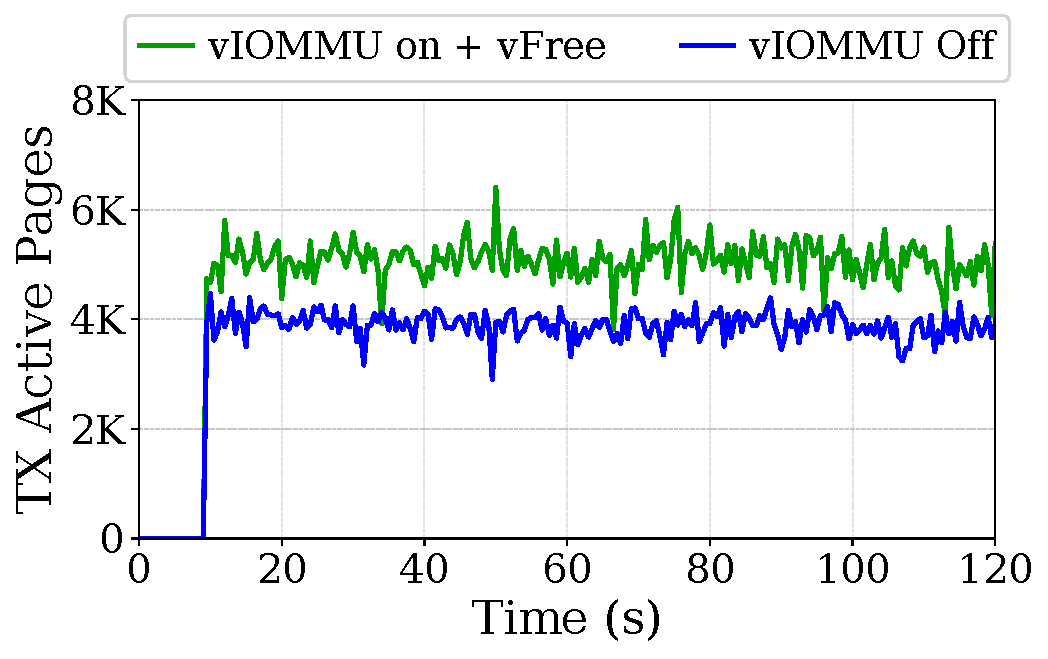
\includegraphics[width=\columnwidth]{figures/tx_mem/mem_fig_tx_active_pages.pdf}
        \Description{Plot showing TX page usage over time.}
        \caption{Active pages required by the Tx datapath over time.}
        \label{vfree:fig:tx_exp_memory_tx}
    \end{subfigure}
    \begin{subfigure}[b]{0.49\columnwidth}
        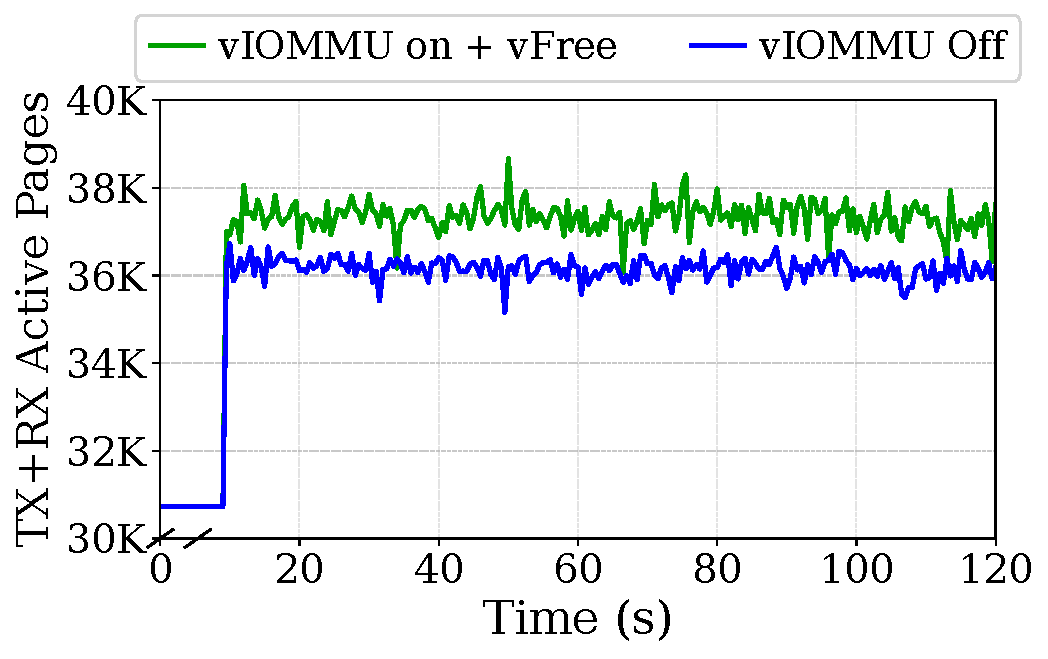
\includegraphics[width=\columnwidth]{figures/tx_mem/mem_fig_tx_rx_active_pages.pdf}
        \Description{Plot showing RX+TX page usage over time.}
        \caption{Active pages required by the Rx and Tx datapath over time.}
        \label{vfree:fig:tx_exp_memory_total}
    \end{subfigure}
    \caption{For Tx-server setup, {\vfreename} incurs less than 3.3\%
     memory overhead over vIOMMU-off.}
    \label{vfree:fig:tx_memory}
\end{figure}

\begin{figure}[!htbp]
    \centering
    \begin{subfigure}[b]{0.49\columnwidth}
        
\includegraphics[width=\columnwidth]{figures/rx_mem/mem_fig_tx_active_pages.pdf}
        \Description{Plot showing TX page usage over time.}
        \caption{Active pages required by the Tx datapath over time.}
        \label{vfree:fig:rx_exp_memory_tx}
    \end{subfigure}
    \begin{subfigure}[b]{0.49\columnwidth}
        
\includegraphics[width=\columnwidth]{figures/rx_mem/mem_fig_tx_rx_active_pages.pdf}
        \Description{Plot showing RX+TX page usage over time.}
        \caption{Active pages required by the Rx and Tx datapath over time.}
        \label{vfree:fig:rx_exp_memory_total}
    \end{subfigure}
    \caption{For Rx-server setup, {\vfreename} incurs less than 2.3\% additional memory overhead over vIOMMU-off.}
    \label{vfree:fig:rx_memory}
\end{figure}

\para{Tx-server.} We measure active physical pages for Tx held by the mlx5 driver. The Tx datapath shows an increase by 30.5\%, an inherent cost of deferring free page (Figure~\ref{vfree:fig:tx_exp_memory_tx}).
However, Figure~\ref{vfree:fig:tx_exp_memory_total} shows that when accounting for both Tx and Rx-datapath active pages, the total page count increases by only 3.28\% over vIOMMU-off,
because the page pool on the Rx side retains pages in its cache rather than actively releasing them to the kernel allocator.

\para{Rx-server.} 
% We measure active page count for Rx using page pool stats~\cite{linux_page_pool,linux_page_pool_stats}.
As shown in Figure~\ref{vfree:fig:rx_exp_memory_total}
\vfreename{} requires only 2.23\% more total pages over vIOMMU-off.
The active page count for Tx datapath only (Figure~\ref{vfree:fig:rx_exp_memory_tx}) shows a larger relative difference,
but memory consumption is dominated by the Rx datapath, so the overall memory overhead is minimal.
